\section{\texorpdfstring{\(\mathbf{R}^n\) 的子群与商群}{R 的 n 次幂的子群与商群}}

让我们首先引进如下的约定：若 G 是一个拓扑群，我们对 n 个都等于 G 的因子的乘积群 \(G^{n}\) （对每个整数 n \textgreater{} 0 ）已经定义过（第 III 章 § 2）。在本节中，我们要把这一定义推广到 n = 0 的情形，约定 \(G^{0}\) 表示只由一个元素组成的群。若 H 是任意群，我们将把 \(G^{0} \times H\) 与 H 等同起来。

\pandocbounded{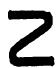
\includegraphics[keepaspectratio]{images/part001_b5dea1c7.jpg}}

在集合 \(\mathbf{R}^n\) 上，我们一方面要考虑它的（加法）拓扑群结构，另一方面要考虑它在域 \(\mathbf{R}\) 上的向量空间结构（第 VI 章 § 1 第 3 小节）。给定子集 \(\mathbf{A}\) （含于 \(\mathbf{R}^n\) ）后，我们可以考虑 \(\mathbf{R}^n\) 的由 \(\mathbf{A}\) 生成的子群（ \(\mathbf{A}\) 的点以整数为系数的一切线性组合所成的集合），同时也可以考虑由 \(\mathbf{A}\) 生成的向量子空间（ \(\mathbf{A}\) 的点以实数为系数的一切线性组合所成的集合）；必须仔细区分这两个概念。按照代数学中作出的定义， \(\mathbf{A}\) 的秩是向量子空间 \(\mathbf{V}\) （ \(\mathbf{R}^n\) 中由 \(\mathbf{A}\) 生成的）的维数；因此说 \(\mathbf{A}\) 的秩为 \(p\) ，就等价于说存在 \(p\) 个点 \(x_i \in \mathbf{A}\) ，它们关于域 \(\mathbf{R}\) 构成一个自由系（换句话说，关系 \(\sum_{i} t_i x_i = 0\) （其中 \(t_i\) 是实数）蕴涵 \(t_i = 0\) （对每个 \(i\) ）），并且构成 \(\mathbf{V}\) 的一个基（意即 \(\mathbf{V}\) 的每个点都是 \(x_i\) 以实数为系数的一个线性组合）。

在以下的内容中，我们还必须用到 \(\mathbf{R}^n\) 的点关于有理数域 \(\mathbf{Q}\) 自由这一概念；这样的系是一个有限子集 \((\pmb{x}_i)\) （ \(\mathbf{R}^n\) 的），满足关系 \(\sum_{i} r_i x_i = 0\) （其中 \(r_i\) 是有理数（或整数——这是一回事））蕴涵对每个 i 有 \(r_{i}=0\) 。这个概念必须与关于 R 的自由系的概念仔细地区分开：每个关于 R 自由的系都关于 Q 自由，但反过来不成立（例如，R 中的数 1 与 \(\sqrt{2}\) 构成关于 Q 的自由系，但不构成关于 R 的自由系）。每当我们不加限定地说到自由系时，总是指关于 R 的自由系。因此有必要在 \(R^{n}\) 上把关于 R 的向量空间结构与关于 Q 的向量空间结构区分开；特别地，由 \(R^{n}\) 的子集 A 生成的关于 Q 的向量子空间是 A 以有理数为系数的一切线性组合所成的集合 U；它含于由 A 生成的（关于 R 的）向量子空间 V，但一般与 V 不同。U（关于 Q）的维数称为 A 的有理秩；它至少等于上面定义的 A 的秩（即 V 关于 R 的维数）；若 A 是无限集，它可以是无限的，而 \(R^{n}\) 的任何非空子集的秩总 \(\leqslant n\) ；特别地， \(R^{n}\) 的任何不可数子集的有理秩总是无限的，因为 Q 上任何有限维向量空间都是可数的。

\pandocbounded{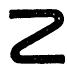
\includegraphics[keepaspectratio]{images/part001_3371d17f.jpg}}

在本节中，我们将首先确定加法群 \(R^{n}\) 的闭子群的结构。

